\chapter{\acl{PPG}}

\acl{PPG} (\acs{PPG}) je neinvazivní, optická metoda, která se využívá k monitorování změn objemu krve v mikrovaskulárním ložisku tkáně, a to v závislosti na čase.
Tato technika je založena na detekci světla absorbovaného nebo odráženého v měřené tkáni, což umožňuje sledovat kardiovaskulární parametry jako je srdeční tep, saturace kyslíkem nebo krevní tlak.
Předností \acs{PPG} je, že se jedná o levnou, neinvazivní metodu měření, i to, že se dá snadno integrovat do nositelných zařízení.
Subjekt může být díky \acs{PPG} dlouhodobě monitorován bez zásahu do běžného života.

Jak je znázorněno na obrázku \ref{fig:snimaniPPG}, základní princip \acs{PPG} spočívá v emisi světla do tkáně a následném měření množství světla, které je od tkáně reflektováno zpět.
Intenzita reflektovaného světla se mění v závislosti na množství krve procházející měřenou oblastí, což je ovlivněno srdečním pumpováním krve.
Tyto změny jsou zaznamenány fotodetektorem a převedeny na elektrický signál, který je dále analyzován \cite{Park2022}.

\begin{figure}[h]
	\centering
	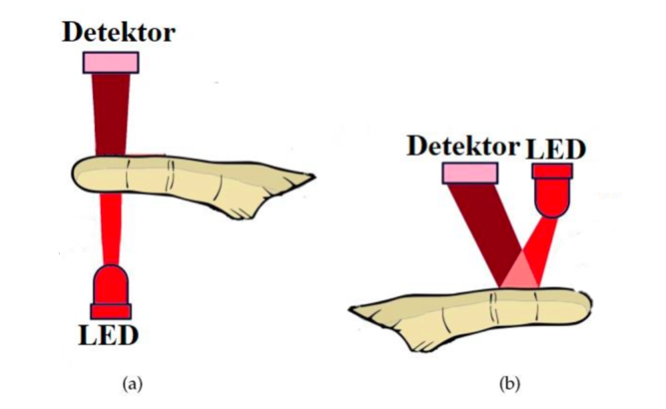
\includegraphics[width=0.8\textwidth]{./obrazky/snimaniPPG.png}
	\caption[Snímání PPG signálu]{Transmisní režim (a) a reflexní režim (b), upraveno z \cite{ENIKÖ}.}
	\label{fig:snimaniPPG}
\end{figure}

\acs{PPG} senzory jsou obvykle umístěny na prstech, uchu nebo na zápěstí, kde mohou efektivně monitorovat průtok krve.

V současné době se \acs{PPG} technologie neustále vyvíjí a rozšiřuje o nové aplikace.
Například, pokročilé algoritmy zpracování signálu a strojové učení otevírají cestu k přesnějšímu a spolehlivějšímu odhadu různých fyziologických parametrů.
Tato vylepšení mají potenciál výrazně zlepšit diagnostiku a monitorování zdravotního stavu v reálném čase.
To může vést ke kvalitnější prevenci a efektivnější léčbě mnoha kardiovaskulárních či respiračních onemocnění.

Tato technologie funguje na fyzikálním principu, při kterém okysličeným hemoglobinem prochází do fotoreceptoru jiná vlnová délka než odkysličeným hemoglobinem \cite{Orphanidou2018}.

% ----------------------------------------------------------------------- %
\section{\acs{PPG} signál}

Obrázek \ref{fig:signalPPG} nám ukazuje, že \acs{PPG} signál vykreslujeme na základě množství světla, které dopadlo na detektor a prošlo skrz tkáň, nebo se od ní odrazilo.
Signál se skládá ze dvou hlavních složek: pulzní (\acs{AC}) složky a ne-pulzní (\acs{DC}) složky.

Pulzní složka (\acs{AC}) \acs{PPG} signálu je synchronní se srdečními cykly a odráží změny objemu krve spojené s každým srdečním cyklem.
Tato složka je pro účel naší práce zásadní.
\acs{AC} složka je ovlivněna cyklickými změnami v objemu arteriální krve pod tlakem srdečních kontrakcí.

Na druhé straně ne-pulzní složka (\acs{DC}) představuje základní hodnotu absorpce světla tkání, která je ovlivněna různými faktory jako například barva kůže, složení tkáně a stabilní objem krve v místě umístěného senzoru.
Dále je ovlivněna vnějšími faktory, jako jsou specifikace měřicí technologie a podmínky okolního osvětlení \cite{ENIKÖ}\cite{Park2022}.

Počátek pulzu v \acs{PPG} signálu je obvykle pozorován v nejnižším bodě předcházejícím systolické fázi, což také odpovídá bodu minimálního objemu krve v tepnách.
Vrchol systolické fáze, představující maximální objem krve, je klíčovým bodem pro analýzu dynamiky průtoku krve.
Po systolickém vrcholu klesá \acs{PPG} signál do diastolické fáze, kde se objevuje výrazný rys známý jako "diastolický zářez".
Tento zářez, následovaný sekundárním vrcholem, indikuje obrácení tlakového gradientu, jak srdeční cyklus pokračuje do diastoly.

Tvar \acs{PPG} vlny se mění na základě vnějších podnětů, fyziologického stavu a složení těla \cite{Park2022}.

\begin{figure}[ht]
	\centering
	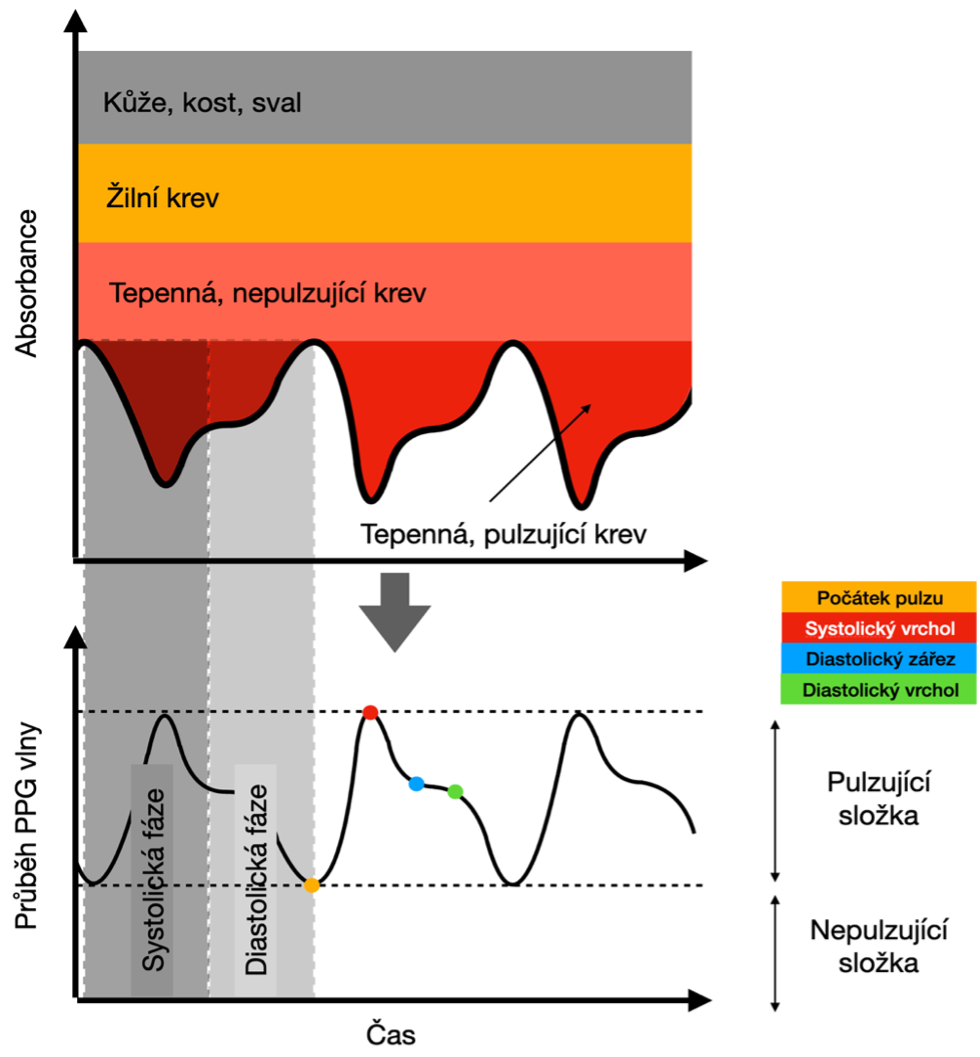
\includegraphics[width=0.8\textwidth]{./obrazky/signalPPG.png}
	\caption[Fiziologický popis PPG signálu]{Princip získání \acs{PPG} křivky a její popis, upraveno z \cite{Park2022}.}
	\label{fig:signalPPG}
\end{figure}